\documentclass{standalone}
\usepackage{tikz}
\usepackage{ctex,siunitx}
\setCJKmainfont{Noto Serif CJK SC}
\usepackage{tkz-euclide}
\usepackage{amsmath}
\usetikzlibrary{patterns, calc}
\usetikzlibrary {decorations.pathmorphing, decorations.pathreplacing, decorations.shapes,}

\begin{document}
\small
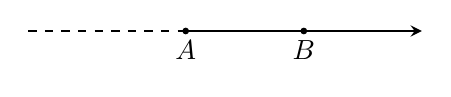
\begin{tikzpicture}[>=stealth,scale=1]
  \tkzSetUpPoint[fill=black]
  % \useasboundingbox(-1,-0.75)rectangle(3.7,1.4);
  \draw[->, thick](0,0)--(3,0);
  \draw[dashed](-2,0)--(0,0);
  \tkzDefPoints{0/0/A,1.5/0/B}
  \tkzDrawPoints(A,B)
  \tkzLabelPoints[below](A,B)
\end{tikzpicture}
\end{document}